\documentclass[11pt, a4paper]{article}

% Mandatory Packages
\usepackage{amsmath}
\usepackage{amssymb}
\usepackage{amsthm}
\usepackage{geometry}
\usepackage{tikz}
\usetikzlibrary{arrows.meta, positioning, shapes, backgrounds}
\usepackage{mathrsfs}
\usepackage{mathtools}
\usepackage{hyperref}
\usepackage{enumitem}

% Page Geometry
\geometry{
    top=1in,
    bottom=1in,
    left=1in,
    right=1in
}

% Theorem Environments
\newtheorem{theorem}{Theorem}[section]
\newtheorem{lemma}[theorem]{Lemma}
\newtheorem{proposition}[theorem]{Proposition}
\newtheorem{corollary}[theorem]{Corollary}
\theoremstyle{definition}
\newtheorem{definition}{Definition}[section]
\newtheorem{axiom}{Axiom}[section]
\newtheorem{example}{Example}[section]
\theoremstyle{remark}
\newtheorem{remark}{Remark}[section]

% Custom Commands for Probability
\newcommand{\E}{\mathbb{E}}
\newcommand{\Var}{\mathrm{Var}}
\newcommand{\Prob}{\mathbb{P}}
\newcommand{\R}{\mathbb{R}}
\newcommand{\N}{\mathbb{N}}
\newcommand{\F}{\mathcal{F}}
\newcommand{\ind}{\mathbf{1}}

\title{\textbf{Homework 3: Moments, Generating Functions, and Tchebysheff's Theorem}}
\author{Tashfeen Omran}
\date{September 2026}

\begin{document}

\maketitle
\tableofcontents
\newpage

% ==========================================
% PART 1: Comprehensive Introduction
% ==========================================
\section{Part 1: Comprehensive Introduction, Context, and Prerequisites}

\subsection{Core Concepts \& Axioms}
In the rigorous study of probability, a random variable $Y$ is not merely a variable that takes on random values, but rather a measurable function mapping a sample space $\Omega$ to the real numbers $\R$, i.e., $Y: (\Omega, \F, \Prob) \to (\R, \mathcal{B}(\R))$. To understand the behavior of $Y$, we often look at its \textit{moments}, which are the expected values of powers of $Y$. 

\begin{definition}[Moments]
The $k$-th moment of a random variable $Y$ about the origin is defined as $\mu'_k = \E[Y^k]$. The $k$-th central moment is defined as $\mu_k = \E[(Y - \mu)^k]$, where $\mu = \mu'_1$.
\end{definition}

To encapsulate all moments into a single mathematical object, we utilize integral transforms. The \textbf{Moment-Generating Function (MGF)} is the Laplace transform of the probability measure, while the \textbf{Probability-Generating Function (PGF)} is closely related to the Z-transform for discrete variables.

\begin{definition}[Moment-Generating Function]
The MGF of a random variable $Y$ is $m(t) = \E[e^{tY}]$, provided there exists a constant $b > 0$ such that the expectation is finite for all $|t| \le b$.
\end{definition}

\begin{definition}[Probability-Generating Function]
For an integer-valued random variable $Y$, the PGF is $P(t) = \E[t^Y] = \sum_{y=0}^\infty p(y) t^y$, for all $t$ such that the sum converges absolutely.
\end{definition}

\subsection{Intuition and Set-Theoretic/Logical Foundations}
Why do we need generating functions? In set-theoretic terms, finding the distribution of a sum of independent random variables $Z = X + Y$ requires computing the convolution of their probability measures: $\Prob(Z = z) = \sum_{x} \Prob(X = x)\Prob(Y = z - x)$. Convolutions are algebraically cumbersome. However, integral transforms map the complex operation of convolution in the probability space to simple pointwise multiplication in the transform space: $m_Z(t) = m_X(t)m_Y(t)$. 

Furthermore, the MGF acts as the "DNA" of a probability distribution. By the Uniqueness Theorem, if two random variables share the same MGF in a neighborhood of zero, their underlying probability measures are identical almost everywhere.

\subsection{Historical Context and Motivation}
The concept of generating functions was pioneered by Abraham de Moivre and Pierre-Simon Laplace in the 18th and 19th centuries to solve linear recurrence relations and formalize the Central Limit Theorem. Later, Pafnuty Chebyshev (Tchebysheff) sought to understand how probability mass concentrates around the mean without knowing the exact distribution. This led to \textbf{Tchebysheff's Theorem}, a foundational result in measure theory that bounds the measure of the tail sets of a distribution, paving the way for the Weak Law of Large Numbers.

\subsection{Key Theorems, Lemmas, and Formulas}
\begin{theorem}[Moment Generation]
If $m(t)$ exists for $|t| \le b$, then $m^{(k)}(0) = \E[Y^k] = \mu'_k$.
\end{theorem}

\begin{theorem}[Factorial Moments via PGF]
If $P(t)$ is the PGF of $Y$, then $P^{(k)}(1) = \E[Y(Y-1)\dots(Y-k+1)] = \mu_{[k]}$.
\end{theorem}

\begin{theorem}[Tchebysheff's Theorem]
Let $Y$ be a random variable with mean $\mu$ and finite variance $\sigma^2$. For any constant $k > 0$:
\[ \Prob(|Y - \mu| \ge k\sigma) \le \frac{1}{k^2} \quad \text{and} \quad \Prob(|Y - \mu| < k\sigma) \ge 1 - \frac{1}{k^2} \]
\end{theorem}

\subsection{Prerequisites}
To master this chapter, one must be proficient in:
\begin{itemize}
    \item \textbf{Real Analysis:} Taylor series expansions (specifically $e^x = \sum x^n/n!$), radius of convergence, and Leibniz's rule for interchanging differentiation and integration/summation.
    \item \textbf{Combinatorics:} The Binomial Theorem $(x+y)^n = \sum \binom{n}{k} x^k y^{n-k}$.
    \item \textbf{Measure Theory Basics:} Understanding expectation as a Lebesgue integral over a probability space.
\end{itemize}

\newpage
% ==========================================
% PART 2: Detailed Homework Solutions
% ==========================================
\section{Part 2: Detailed Homework Solutions (Rigorous Proofs \& Computations)}

\textit{Note: Problems have been strategically selected to cover all distinct archetypes: MGF derivation, Moment extraction, Linear Transformations, PGF derivation, and Concentration Inequalities.}

\subsection{Problem 3.145: Derivation of the Binomial MGF}
\textbf{Problem Statement:} If $Y$ has a binomial distribution with $n$ trials and probability of success $p$, show that the moment-generating function for $Y$ is $m(t) = (pe^t + q)^n$, where $q = 1 - p$.

\begin{proof}[Direct Proof]
Let $Y \sim \text{Binomial}(n, p)$. The probability mass function (PMF) of $Y$ is given by:
\[ p(y) = \binom{n}{y} p^y q^{n-y}, \quad \text{for } y \in \{0, 1, \dots, n\} \]
By Definition 3.14, the moment-generating function is the expectation of $e^{tY}$:
\begin{align*}
    m(t) &= \E[e^{tY}] \\
         &= \sum_{y=0}^{n} e^{ty} p(y) \quad \text{(by the Law of the Unconscious Statistician)} \\
         &= \sum_{y=0}^{n} e^{ty} \binom{n}{y} p^y q^{n-y} \\
         &= \sum_{y=0}^{n} \binom{n}{y} (pe^t)^y q^{n-y} \quad \text{(grouping terms with power } y \text{)}
\end{align*}
We now invoke the Binomial Theorem, which states that for any real numbers $a$ and $b$, $(a+b)^n = \sum_{y=0}^n \binom{n}{y} a^y b^{n-y}$. Let $a = pe^t$ and $b = q$. Substituting these into the theorem yields:
\[ m(t) = (pe^t + q)^n \]
This sum is finite, hence it converges for all $t \in \R$. 
\end{proof}

\subsection{Problem 3.146: Moment Extraction via MGF}
\textbf{Problem Statement:} Differentiate the moment-generating function in Exercise 3.145 to find $\E(Y)$ and $\E(Y^2)$. Then find $\Var(Y)$.

\begin{proof}[Computational Proof]
We are given $m(t) = (pe^t + q)^n$. By Theorem 3.12, $\E(Y) = m'(0)$ and $\E(Y^2) = m''(0)$.

\textbf{Step 1: First Derivative and Expected Value}
Using the chain rule:
\begin{align*}
    m'(t) &= \frac{d}{dt} \left[ (pe^t + q)^n \right] \\
          &= n(pe^t + q)^{n-1} \cdot \frac{d}{dt}(pe^t + q) \\
          &= n(pe^t + q)^{n-1} (pe^t)
\end{align*}
Evaluating at $t = 0$:
\begin{align*}
    \E(Y) &= m'(0) = n(pe^0 + q)^{n-1} (pe^0) \\
          &= n(p + q)^{n-1} p
\end{align*}
Since $p + q = 1$, we have $1^{n-1} = 1$. Thus:
\[ \E(Y) = np \]

\textbf{Step 2: Second Derivative and Second Moment}
We differentiate $m'(t)$ using the product rule and chain rule. Let $u(t) = n(pe^t + q)^{n-1}$ and $v(t) = pe^t$.
\begin{align*}
    m''(t) &= u'(t)v(t) + u(t)v'(t) \\
           &= \left[ n(n-1)(pe^t + q)^{n-2}(pe^t) \right] (pe^t) + \left[ n(pe^t + q)^{n-1} \right] (pe^t) \\
           &= n(n-1)(pe^t + q)^{n-2}(p^2 e^{2t}) + n(pe^t + q)^{n-1}(pe^t)
\end{align*}
Evaluating at $t = 0$:
\begin{align*}
    \E(Y^2) &= m''(0) = n(n-1)(p + q)^{n-2}(p^2) + n(p + q)^{n-1}(p) \\
            &= n(n-1)p^2 + np \quad \text{(since } p+q=1 \text{)} \\
            &= n^2p^2 - np^2 + np
\end{align*}

\textbf{Step 3: Variance Calculation}
By definition, $\Var(Y) = \E(Y^2) - [\E(Y)]^2$.
\begin{align*}
    \Var(Y) &= (n^2p^2 - np^2 + np) - (np)^2 \\
            &= n^2p^2 - np^2 + np - n^2p^2 \\
            &= np - np^2 \\
            &= np(1 - p) \\
            &= npq
\end{align*}
\end{proof}

\subsection{Problem 3.158: Linear Transformations of MGFs}
\textbf{Problem Statement:} If $Y$ is a random variable with MGF $m(t)$ and if $W = aY + b$, show that the MGF of $W$ is $e^{tb}m(at)$.

\begin{proof}[Direct Proof]
By Definition 3.14, the MGF of $W$ is:
\begin{align*}
    m_W(t) &= \E[e^{tW}] \\
           &= \E[e^{t(aY + b)}] \quad \text{(substituting } W = aY + b \text{)} \\
           &= \E[e^{atY + bt}] \\
           &= \E[e^{bt} e^{(at)Y}] \quad \text{(properties of exponents)}
\end{align*}
Since $e^{bt}$ is a deterministic constant with respect to the expectation operator (which integrates over the probability space of $Y$), we can factor it out by the linearity of expectation:
\begin{align*}
    m_W(t) &= e^{bt} \E[e^{(at)Y}]
\end{align*}
Recognizing that $\E[e^{(at)Y}]$ is exactly the definition of the MGF of $Y$ evaluated at the parameter $(at)$, we conclude:
\[ m_W(t) = e^{tb} m_Y(at) \]
\end{proof}

\subsection{Problem 3.159: Moments of Linear Transformations}
\textbf{Problem Statement:} Use the result in Exercise 3.158 to prove that, if $W = aY + b$, then $\E(W) = a\E(Y) + b$ and $\Var(W) = a^2\Var(Y)$.

\begin{proof}[Direct Proof]
From 3.158, $m_W(t) = e^{tb} m_Y(at)$. We find the moments by differentiating with respect to $t$.

\textbf{Step 1: Expected Value}
Using the product rule and chain rule:
\begin{align*}
    m_W'(t) &= \frac{d}{dt} \left[ e^{tb} m_Y(at) \right] \\
            &= b e^{tb} m_Y(at) + e^{tb} \cdot m_Y'(at) \cdot a
\end{align*}
Evaluating at $t = 0$:
\begin{align*}
    \E(W) &= m_W'(0) = b e^0 m_Y(0) + a e^0 m_Y'(0)
\end{align*}
Since $m_Y(0) = \E[e^0] = 1$ and $m_Y'(0) = \E(Y)$, we have:
\[ \E(W) = b(1) + a\E(Y) = a\E(Y) + b \]

\textbf{Step 2: Variance}
We differentiate $m_W'(t)$ again:
\begin{align*}
    m_W''(t) &= \frac{d}{dt} \left[ b e^{tb} m_Y(at) + a e^{tb} m_Y'(at) \right] \\
             &= \left[ b^2 e^{tb} m_Y(at) + ab e^{tb} m_Y'(at) \right] + \left[ ab e^{tb} m_Y'(at) + a^2 e^{tb} m_Y''(at) \right] \\
             &= b^2 e^{tb} m_Y(at) + 2ab e^{tb} m_Y'(at) + a^2 e^{tb} m_Y''(at)
\end{align*}
Evaluating at $t = 0$:
\begin{align*}
    \E(W^2) &= m_W''(0) = b^2(1) + 2ab\E(Y) + a^2\E(Y^2)
\end{align*}
Now, compute the variance:
\begin{align*}
    \Var(W) &= \E(W^2) - [\E(W)]^2 \\
            &= \left( b^2 + 2ab\E(Y) + a^2\E(Y^2) \right) - \left( a\E(Y) + b \right)^2 \\
            &= b^2 + 2ab\E(Y) + a^2\E(Y^2) - \left( a^2[\E(Y)]^2 + 2ab\E(Y) + b^2 \right) \\
            &= a^2\E(Y^2) - a^2[\E(Y)]^2 \\
            &= a^2 \left( \E(Y^2) - [\E(Y)]^2 \right) \\
            &= a^2 \Var(Y)
\end{align*}
\end{proof}

\subsection{Problem 3.165: Probability-Generating Function for Poisson}
\textbf{Problem Statement:} Let $Y$ denote a Poisson random variable with mean $\lambda$. Find the probability-generating function for $Y$ and use it to find $\E(Y)$ and $\Var(Y)$.

\begin{proof}[Direct Proof]
The PMF of a Poisson random variable is $p(y) = \frac{\lambda^y e^{-\lambda}}{y!}$ for $y \in \{0, 1, 2, \dots\}$.
By Definition 3.15, the PGF is:
\begin{align*}
    P(t) &= \E[t^Y] = \sum_{y=0}^{\infty} t^y \frac{\lambda^y e^{-\lambda}}{y!} \\
         &= e^{-\lambda} \sum_{y=0}^{\infty} \frac{(\lambda t)^y}{y!}
\end{align*}
Recognizing the Taylor series expansion for the exponential function, $\sum_{y=0}^\infty \frac{x^y}{y!} = e^x$, we substitute $x = \lambda t$:
\begin{align*}
    P(t) &= e^{-\lambda} e^{\lambda t} = e^{\lambda(t - 1)}
\end{align*}

To find the moments, we use Theorem 3.13: $P^{(k)}(1) = \E[Y(Y-1)\dots(Y-k+1)]$.
First derivative:
\[ P'(t) = \frac{d}{dt} e^{\lambda(t-1)} = \lambda e^{\lambda(t-1)} \]
Evaluating at $t=1$:
\[ \E(Y) = P'(1) = \lambda e^0 = \lambda \]

Second derivative:
\[ P''(t) = \frac{d}{dt} \left[ \lambda e^{\lambda(t-1)} \right] = \lambda^2 e^{\lambda(t-1)} \]
Evaluating at $t=1$:
\[ \E[Y(Y-1)] = P''(1) = \lambda^2 e^0 = \lambda^2 \]
Notice that $\E[Y(Y-1)] = \E(Y^2) - \E(Y)$. Therefore, $\E(Y^2) = \lambda^2 + \E(Y) = \lambda^2 + \lambda$.
Finally, the variance is:
\begin{align*}
    \Var(Y) &= \E(Y^2) - [\E(Y)]^2 \\
            &= (\lambda^2 + \lambda) - \lambda^2 \\
            &= \lambda
\end{align*}
\end{proof}

\subsection{Problem 3.167: Tchebysheff's Theorem Application}
\textbf{Problem Statement:} Let $Y$ be a random variable with mean 11 and variance 9. Using Tchebysheff's theorem, find:
(a) a lower bound for $\Prob(6 < Y < 16)$.
(b) the value of $C$ such that $\Prob(|Y - 11| \ge C) \le .09$.

\begin{proof}[Computational Proof]
We are given $\mu = 11$ and $\sigma^2 = 9$, which implies $\sigma = 3$.

\textbf{Part (a):} We want to bound $\Prob(6 < Y < 16)$.
Notice that the interval $(6, 16)$ is symmetric about the mean $\mu = 11$.
\[ 6 < Y < 16 \iff -5 < Y - 11 < 5 \iff |Y - 11| < 5 \]
We set this equal to the Tchebysheff format $|Y - \mu| < k\sigma$:
\[ k\sigma = 5 \implies k(3) = 5 \implies k = \frac{5}{3} \]
By Theorem 3.14, the lower bound is:
\[ \Prob(|Y - 11| < 5) \ge 1 - \frac{1}{k^2} = 1 - \frac{1}{(5/3)^2} = 1 - \frac{9}{25} = \frac{16}{25} = 0.64 \]

\textbf{Part (b):} We want $C$ such that $\Prob(|Y - 11| \ge C) \le 0.09$.
By Tchebysheff's theorem, $\Prob(|Y - \mu| \ge k\sigma) \le \frac{1}{k^2}$.
We equate the upper bound to $0.09$:
\[ \frac{1}{k^2} = 0.09 = \frac{9}{100} \implies k^2 = \frac{100}{9} \implies k = \frac{10}{3} \]
The constant $C$ corresponds to $k\sigma$:
\[ C = k\sigma = \left(\frac{10}{3}\right)(3) = 10 \]
\end{proof}

\subsection{Problem 3.169: Tightness of Tchebysheff's Bound}
\textbf{Problem Statement:} Let $Y$ have PMF $p(-1) = 1/18$, $p(0) = 16/18$, $p(1) = 1/18$.
(a) Show $\E(Y) = 0$ and $\Var(Y) = 1/9$.
(b) Calculate $\Prob(|Y - \mu| \ge 3\sigma)$ and compare to Tchebysheff's bound for $k=3$.
(c) Construct a distribution for $X$ such that $\Prob(|X - \mu_X| \ge 2\sigma_X) = 1/4$.

\begin{proof}[Direct Proof]
\textbf{Part (a):}
\begin{align*}
    \E(Y) &= \sum y p(y) = (-1)\left(\frac{1}{18}\right) + (0)\left(\frac{16}{18}\right) + (1)\left(\frac{1}{18}\right) = 0 \\
    \E(Y^2) &= \sum y^2 p(y) = (-1)^2\left(\frac{1}{18}\right) + (0)^2\left(\frac{16}{18}\right) + (1)^2\left(\frac{1}{18}\right) = \frac{2}{18} = \frac{1}{9} \\
    \Var(Y) &= \E(Y^2) - [\E(Y)]^2 = \frac{1}{9} - 0 = \frac{1}{9}
\end{align*}

\textbf{Part (b):}
Since $\Var(Y) = 1/9$, $\sigma = 1/3$. We want $\Prob(|Y - 0| \ge 3(1/3)) = \Prob(|Y| \ge 1)$.
The only values $Y$ takes that satisfy $|Y| \ge 1$ are $-1$ and $1$.
\[ \Prob(|Y| \ge 1) = p(-1) + p(1) = \frac{1}{18} + \frac{1}{18} = \frac{2}{18} = \frac{1}{9} \]
Tchebysheff's bound for $k=3$ states $\Prob(|Y - \mu| \ge 3\sigma) \le 1/3^2 = 1/9$.
The exact probability equals the upper bound, proving that Tchebysheff's inequality is \textit{tight} (cannot be improved without further assumptions).

\textbf{Part (c):}
We want to construct $X$ such that $\Prob(|X - \mu_X| \ge 2\sigma_X) = 1/4$.
Assume a symmetric distribution $X \in \{-1, 0, 1\}$ with $p(-1) = p$, $p(1) = p$, and $p(0) = 1 - 2p$.
By symmetry, $\mu_X = 0$.
The variance is $\sigma_X^2 = (-1)^2 p + (0)^2(1-2p) + (1)^2 p = 2p$. Thus, $\sigma_X = \sqrt{2p}$.
We require $\Prob(|X| \ge 2\sqrt{2p}) = 1/4$.
Assume $2\sqrt{2p} \le 1$. Then the event $|X| \ge 2\sqrt{2p}$ includes exactly the outcomes $X = -1$ and $X = 1$.
The probability of this event is $p(-1) + p(1) = 2p$.
Setting this equal to the desired probability:
\[ 2p = \frac{1}{4} \implies p = \frac{1}{8} \]
Let us verify the assumption: $2\sqrt{2(1/8)} = 2\sqrt{1/4} = 2(1/2) = 1 \le 1$. The assumption holds.
Thus, the distribution is $p(-1) = 1/8$, $p(1) = 1/8$, $p(0) = 3/4$.
\end{proof}

\newpage
% ==========================================
% PART 3: In-Depth Analysis
% ==========================================
\section{Part 3: In-Depth Analysis of Problems and Techniques}

\subsection{A) Problem Types and Logical Strategies}
\begin{itemize}
    \item \textbf{Transform Derivations (Problems 3.145, 3.165):} The strategy is to write out the expectation as an infinite sum (or integral) and algebraically manipulate it into a known Taylor series (like $e^x$) or a Binomial expansion. The goal is to collapse the infinite series into a closed-form function of $t$.
    \item \textbf{Moment Extraction via Calculus (Problems 3.146, 3.165):} Once a closed-form MGF or PGF is found, moments are extracted by taking derivatives. The overarching strategy is to use the Chain Rule and Product Rule meticulously, and then evaluate at $t=0$ (for MGFs) or $t=1$ (for PGFs).
    \item \textbf{Linear Transformations (Problems 3.158, 3.159):} These proofs rely on the linearity of the expectation operator. The strategy is to substitute the linear equation into the exponent of the MGF definition and factor out deterministic constants.
    \item \textbf{Concentration Inequalities (Problems 3.167, 3.169):} These problems require mapping a specific probability interval to the abstract form $|Y - \mu| < k\sigma$. The strategy is algebraic matching: find $\mu$ and $\sigma$, set the boundary equal to $k\sigma$, solve for $k$, and apply the $1/k^2$ bound.
\end{itemize}

\subsection{B) Key Analytical and Logical Manipulations}
\begin{itemize}
    \item \textbf{The Law of the Unconscious Statistician (LOTUS):} Used implicitly in 3.145 and 3.165. It allows us to compute $\E[g(Y)]$ directly using the PMF of $Y$, rather than finding the distribution of $g(Y)$ first.
    \item \textbf{Taylor Series Recognition:} In 3.165, recognizing that $\sum (\lambda t)^y / y!$ is the Maclaurin series for $e^{\lambda t}$ is the critical algebraic trick that collapses the infinite sum.
    \item \textbf{Factorial Moment Adjustment:} In 3.165, the PGF yields $\E[Y(Y-1)]$. A common logical manipulation is expanding this to $\E[Y^2] - \E[Y]$ and rearranging to isolate $\E[Y^2]$, which is strictly necessary to compute the variance.
    \item \textbf{Symmetry Arguments:} In 3.169(c), assuming a symmetric distribution centered at zero drastically reduced the parameter space, forcing $\mu=0$ and making the variance a simple function of a single probability $p$.
\end{itemize}

\newpage
% ==========================================
% PART 4: Cheatsheet, Visuals, and Tips
% ==========================================
\section{Part 4: "Cheatsheet", Visuals, and Tips for Success}

\subsection{Theorems \& Equivalences Summary}
\begin{table}[h!]
\centering
\renewcommand{\arraystretch}{1.5}
\begin{tabular}{|l|l|l|}
\hline
\textbf{Concept} & \textbf{Definition / Formula} & \textbf{Key Property} \\ \hline
MGF & $m(t) = \E[e^{tY}]$ & $m^{(k)}(0) = \E[Y^k]$ \\ \hline
PGF & $P(t) = \E[t^Y]$ & $P^{(k)}(1) = \E[Y(Y-1)\dots(Y-k+1)]$ \\ \hline
Variance via MGF & $\Var(Y) = m''(0) - [m'(0)]^2$ & Requires evaluating at $t=0$ \\ \hline
Variance via PGF & $\Var(Y) = P''(1) + P'(1) - [P'(1)]^2$ & Requires evaluating at $t=1$ \\ \hline
Tchebysheff & $\Prob(|Y - \mu| \ge k\sigma) \le \frac{1}{k^2}$ & Universal bound for any distribution \\ \hline
\end{tabular}
\end{table}

\subsection{Set \& Logic Illustrations: The Transform Mapping}
The following TikZ diagram illustrates how integral transforms map operations from the Probability Space (where convolutions are hard) to the Transform Space (where multiplication is easy).

\begin{center}
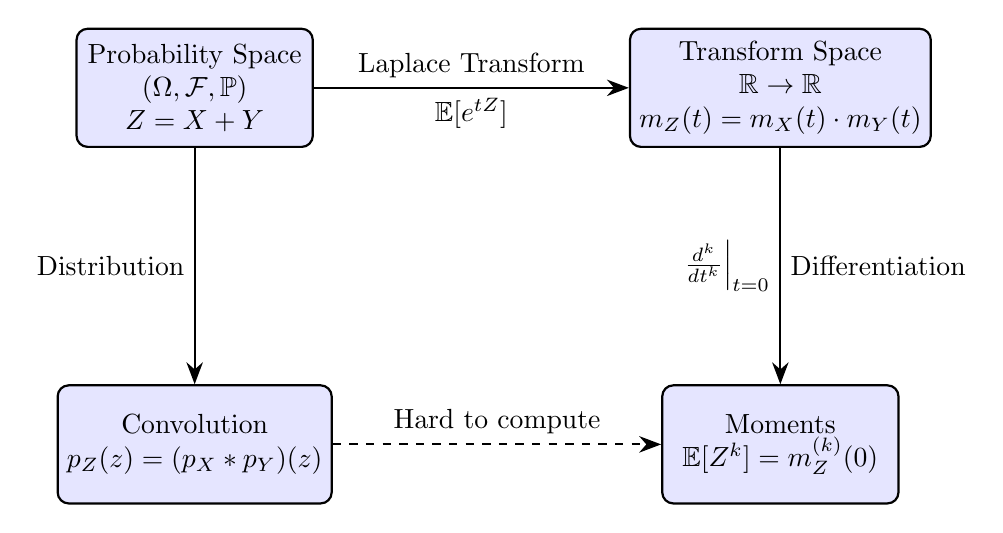
\begin{tikzpicture}[
    node distance=3cm and 4cm,
    box/.style={rectangle, draw=black, thick, fill=blue!10, minimum width=3cm, minimum height=1.5cm, align=center, rounded corners},
    arrow/.style={-{Stealth[scale=1.2]}, thick, draw=black}
]

% Nodes
\node[box] (prob) {Probability Space \\ $(\Omega, \F, \Prob)$ \\ $Z = X + Y$};
\node[box, right=of prob] (trans) {Transform Space \\ $\R \to \R$ \\ $m_Z(t) = m_X(t) \cdot m_Y(t)$};
\node[box, below=of prob] (conv) {Convolution \\ $p_Z(z) = (p_X * p_Y)(z)$};
\node[box, below=of trans] (moments) {Moments \\ $\E[Z^k] = m_Z^{(k)}(0)$};

% Arrows
\draw[arrow] (prob) -- node[above] {Laplace Transform} node[below] {$\E[e^{tZ}]$} (trans);
\draw[arrow] (prob) -- node[left] {Distribution} (conv);
\draw[arrow] (trans) -- node[right] {Differentiation} node[left] {$\frac{d^k}{dt^k} \Big|_{t=0}$} (moments);
\draw[arrow, dashed] (conv) -- node[above] {Hard to compute} (moments);

\end{tikzpicture}
\end{center}

\subsection{Heuristics \& "Cheats"}
\begin{itemize}
    \item \textbf{The "Discrete Integer" Cheat:} If a random variable represents counts (e.g., Binomial, Poisson, Geometric), the PGF is almost always algebraically easier to derive and differentiate than the MGF.
    \item \textbf{The "Linear Shift" Trick:} If you need the MGF of $Y - \mu$, use the linear transformation rule: $m_{Y-\mu}(t) = e^{-\mu t}m_Y(t)$. This directly generates \textit{central moments} upon differentiation.
\end{itemize}

\subsection{Pitfalls \& Fallacies}
\begin{itemize}
    \item \textbf{The Evaluation Fallacy:} A very common mistake is finding the derivative $m'(t)$ and forgetting to evaluate it at $t=0$. $m'(t)$ is a function, not a scalar moment.
    \item \textbf{The PGF Variance Trap:} Students often compute variance from a PGF as $P''(1) - [P'(1)]^2$. This is mathematically false. Because $P''(1) = \E[Y^2] - \E[Y]$, you must \textit{add back} $P'(1)$ before subtracting the squared mean.
    \item \textbf{Tchebysheff Misinterpretation:} Applying Tchebysheff for $k \le 1$. If $k=1$, the bound is $\Prob(|Y-\mu| \ge \sigma) \le 1$, which is trivially true for all probabilities and provides zero new information.
\end{itemize}

\newpage
% ==========================================
% PART 5: Conceptual Synthesis
% ==========================================
\section{Part 5: Conceptual Synthesis and The "Big Picture"}

\subsection{A) Thematic Connections}
The core theme of this chapter is \textbf{analytical isomorphism}. We are establishing a structural mapping between the space of probability measures and the space of analytic functions. By mapping a probability distribution to an MGF, we translate the probabilistic concept of "expected value" into the calculus concept of "derivatives at the origin." This unifies previous topics: the discrete summations and continuous integrals used to find expected values in earlier chapters are now seen as special cases of evaluating a single, unified generating function.

\subsection{B) Forward and Backward Links}
\textbf{Backward Links:} This topic builds directly on the Law of the Unconscious Statistician (LOTUS) and the linearity of expectation. It formalizes why we spent time learning to compute $\E[g(Y)]$ for arbitrary functions $g$.

\textbf{Forward Links:} Understanding MGFs is the absolute bedrock for advanced probability. In future chapters, the \textbf{Central Limit Theorem (CLT)} is proven not by looking at PDFs, but by showing that the MGF of a standardized sample mean converges pointwise to $e^{t^2/2}$, which is the MGF of the Standard Normal distribution. Furthermore, Tchebysheff's inequality is the gateway to \textbf{Measure Theory} and \textbf{Large Deviations Theory}, serving as the foundational logic for proving the Weak Law of Large Numbers (WLLN).

% ==========================================
% PART 6: Abstract Real-World Modeling
% ==========================================
\section{Part 6: Abstract Real-World Modeling (AI, ML, \& Quant Finance)}

\subsection{A) Concrete Scenarios}
\begin{enumerate}
    \item \textbf{Quantitative Finance (Value at Risk - VaR):} In algorithmic trading, assuming asset returns follow a Normal distribution is a fatal flaw (due to "fat tails"). Quants use Tchebysheff's inequality to establish distribution-free bounds on the Value at Risk. Even if the true market distribution is unknown, Tchebysheff guarantees the maximum probability of a catastrophic loss exceeding $k$ standard deviations.
    \item \textbf{Machine Learning (PAC Learning Bounds):} In Statistical Learning Theory, we must prove that a model's empirical training error converges to its true generalization error. This is done using Chernoff Bounds, which are derived directly by applying Markov's Inequality to the Moment-Generating Function of the loss variables.
\end{enumerate}

\subsection{B) Model Problem Setup: Chernoff Bounds in ML}
Let us build a rigorous mathematical model for bounding generalization error in Machine Learning using MGFs.

\textbf{State Space \& Random Variables:} Let $\mathcal{D}$ be an unknown probability distribution over a feature space $\mathcal{X} \times \mathcal{Y}$. Let our ML model be a hypothesis $h: \mathcal{X} \to \mathcal{Y}$. We define a loss function $L(h(x), y) \in [0, 1]$. 
Let $Z_i = L(h(x_i), y_i)$ be independent, identically distributed random variables representing the loss on the $i$-th training example, with true expected risk $\mu = \E[Z_i]$.

\textbf{The Optimization Problem:} We observe the empirical risk $\hat{\mu} = \frac{1}{n} \sum_{i=1}^n Z_i$. We want to bound the probability that our empirical risk severely underestimates the true risk: $\Prob(\hat{\mu} - \mu \ge \epsilon)$.

\textbf{Theoretical Framework (Using MGFs):}
For any $t > 0$, the function $e^{tx}$ is strictly monotonically increasing. Thus, the event $\{\hat{\mu} - \mu \ge \epsilon\}$ is strictly equivalent to $\{e^{t(\hat{\mu} - \mu)} \ge e^{t\epsilon}\}$.
By Markov's Inequality (the generalized form of Tchebysheff's):
\[ \Prob(\hat{\mu} - \mu \ge \epsilon) = \Prob(e^{t(\hat{\mu} - \mu)} \ge e^{t\epsilon}) \le \frac{\E[e^{t(\hat{\mu} - \mu)}]}{e^{t\epsilon}} \]
The numerator is exactly the MGF of the centered empirical risk! Because the $Z_i$ are independent, the MGF of the sum factors into the product of the individual MGFs. By optimizing the parameter $t$ (finding the infimum over $t > 0$), we derive the \textbf{Chernoff Bound}, proving that the probability of a large generalization gap decays exponentially with the number of training samples $n$. This proves why deep learning requires massive datasets.

\newpage
% ==========================================
% PART 7: Common Variations and Untested Concepts
% ==========================================
\section{Part 7: Common Variations and Untested Concepts}

\subsection{The Characteristic Function (When MGFs Fail)}
A critical edge-case not covered in the standard homework is the \textbf{existence} of the MGF. The definition requires $\E[e^{tY}] < \infty$ for $|t| \le b$. However, for heavy-tailed distributions (like the Cauchy or Log-Normal distributions), the integral diverges, meaning the MGF \textit{does not exist}. 

To solve this, advanced probability theory introduces the \textbf{Characteristic Function}, defined using complex analysis:
\[ \phi_Y(t) = \E[e^{itY}] = \E[\cos(tY)] + i\E[\sin(tY)] \]
Because $|e^{itY}| = 1$, the characteristic function is bounded and is guaranteed to exist for \textit{every} valid probability distribution.

\begin{example}[Proof of Characteristic Function Boundedness]
Let $Y$ be any random variable with probability measure $\mu_Y$.
\begin{align*}
    |\phi_Y(t)| &= \left| \int_{\R} e^{ity} d\mu_Y(y) \right| \\
                &\le \int_{\R} \left| e^{ity} \right| d\mu_Y(y) \quad \text{(by the Triangle Inequality for Integrals)} \\
                &= \int_{\R} 1 \, d\mu_Y(y) \quad \text{(since } |e^{i\theta}| = \sqrt{\cos^2\theta + \sin^2\theta} = 1 \text{)} \\
                &= 1
\end{align*}
Thus, $\phi_Y(t)$ is uniformly bounded by 1 and exists everywhere, unlike the MGF.
\end{example}

% ==========================================
% PART 8: Advanced Diagnostic Testing
% ==========================================
\section{Part 8: Advanced Diagnostic Testing: "Find the Flaw"}

Below are five advanced proofs. Each contains a single, subtle, yet critical mathematical flaw. Act as the grader to find the error.

\subsection{Flawed Proofs}

\textbf{Problem 1:} Let $Y$ be a random variable. We wish to find the MGF of $X = \ln(Y)$.
\begin{proof}
By definition, $m_X(t) = \E[e^{tX}]$. Substituting $X = \ln(Y)$, we get $m_X(t) = \E[e^{t \ln(Y)}]$. Using logarithm rules, $e^{t \ln(Y)} = e^{\ln(Y^t)} = Y^t$. Therefore, $m_X(t) = \E[Y^t]$. We have successfully found the MGF.
\end{proof}

\textbf{Problem 2:} Let $Y$ have PGF $P(t)$. We wish to prove that $\Var(Y) = P''(1) - [P'(1)]^2$.
\begin{proof}
We know that $\Var(Y) = \E(Y^2) - [\E(Y)]^2$.
By Theorem 3.13, $P'(1) = \E(Y)$ and $P''(1) = \E(Y^2)$.
Substituting these directly into the variance formula yields $\Var(Y) = P''(1) - [P'(1)]^2$.
\end{proof}

\textbf{Problem 3:} Let $X$ and $Y$ be random variables such that $m_X(t) = m_Y(t)$ for all $t \in (-1, 1)$. Prove that $\Prob(X = Y) = 1$.
\begin{proof}
By the Uniqueness Theorem of Moment-Generating Functions, if two random variables have the same MGF in a neighborhood around zero, they are the same random variable. Since $(-1, 1)$ is a neighborhood around zero, $X$ and $Y$ are identical. Therefore, the probability that they equal each other is 1, i.e., $\Prob(X = Y) = 1$.
\end{proof}

\textbf{Problem 4:} Use Tchebysheff's inequality to bound the probability that a standard normal random variable $Z \sim N(0,1)$ falls within 0.5 standard deviations of the mean.
\begin{proof}
We want to find a lower bound for $\Prob(|Z - 0| < 0.5(1))$.
Using Tchebysheff's Theorem with $k = 0.5$:
$\Prob(|Z| < 0.5) \ge 1 - \frac{1}{(0.5)^2} = 1 - \frac{1}{0.25} = 1 - 4 = -3$.
Thus, the probability is at least -3.
\end{proof}

\textbf{Problem 5:} Let $X$ be a random variable. Prove that $\E[e^{tX}] = e^{t\E[X]}$.
\begin{proof}
Let $\mu = \E[X]$. We evaluate the expectation of the exponential function. Since the exponential function is continuous and smooth, we can pass the expectation operator inside the function argument. Therefore, $\E[e^{tX}] = e^{\E[tX]}$. By linearity of expectation, $\E[tX] = t\E[X]$. Thus, $\E[e^{tX}] = e^{t\E[X]}$.
\end{proof}

\newpage
\subsection{Solution Key: Resolutions to Flawed Proofs}

\textbf{Resolution 1:} 
\textit{Flaw:} The algebraic manipulation is correct, but the conclusion is a misinterpretation. $\E[Y^t]$ is the definition of the $t$-th \textit{fractional moment} of $Y$, not an MGF in standard form. Furthermore, $Y$ must be strictly positive almost surely for $\ln(Y)$ to be defined, which was not stated in the assumptions.

\textbf{Resolution 2:}
\textit{Flaw:} The statement $P''(1) = \E(Y^2)$ is mathematically false. By Theorem 3.13, $P''(1)$ yields the second \textit{factorial} moment, $\E[Y(Y-1)] = \E(Y^2) - \E(Y)$. To get $\E(Y^2)$, one must compute $P''(1) + P'(1)$. The correct variance formula is $\Var(Y) = P''(1) + P'(1) - [P'(1)]^2$.

\textbf{Resolution 3:}
\textit{Flaw:} The Uniqueness Theorem implies equality \textit{in distribution}, not equality \textit{almost surely}. $m_X(t) = m_Y(t)$ means $F_X(z) = F_Y(z)$ for all $z$. It does NOT mean $X(\omega) = Y(\omega)$ for the underlying sample space. For example, if $X \sim N(0,1)$ and $Y = -X$, they have the exact same MGF, but $\Prob(X = Y) = \Prob(X = -X) = \Prob(X = 0) = 0$.

\textbf{Resolution 4:}
\textit{Flaw:} Tchebysheff's inequality is only useful and meaningful for $k > 1$. While the algebraic statement $\Prob \ge -3$ is technically true (since all probabilities are $\ge 0$, and $0 \ge -3$), it is a vacuous truth that provides zero mathematical insight. The flaw is applying the theorem outside its domain of practical utility.

\textbf{Resolution 5:}
\textit{Flaw:} The proof falsely assumes that expectation commutes with non-linear functions ($\E[g(X)] = g(\E[X])$). This is a severe violation of \textbf{Jensen's Inequality}. Because $g(x) = e^{tx}$ is a strictly convex function, Jensen's Inequality dictates that $\E[e^{tX}] \ge e^{t\E[X]}$, with equality holding if and only if $X$ is a deterministic constant.

\end{document}